% Fig. 3 -- indoor semantic stability.
% ============================ LAYOUT TEMPLATE ============================
% The per-frame label sequence is NOT yet measured: no stored run persists it
% (results/2026-08-26_qualitative_figure_mining_v01/FIGURE_SHORTLIST.md, Fig. 3
% section). The label cells below are deliberately drawn as unknown, and the
% number of label runs is taken from the measured switch count, not invented.
% Do NOT publish this with guessed class names. When
% mining_scripts/run_fig3_replay.pbs has run, replace the "?" chips with the
% recorded labels and delete the template banner.
% ========================================================================
% Paste-ready TikZ body. Include from sec/*.tex with:
%   % Fig. 3 -- indoor semantic stability.
% ============================ LAYOUT TEMPLATE ============================
% The per-frame label sequence is NOT yet measured: no stored run persists it
% (results/2026-08-26_qualitative_figure_mining_v01/FIGURE_SHORTLIST.md, Fig. 3
% section). The label cells below are deliberately drawn as unknown, and the
% number of label runs is taken from the measured switch count, not invented.
% Do NOT publish this with guessed class names. When
% mining_scripts/run_fig3_replay.pbs has run, replace the "?" chips with the
% recorded labels and delete the template banner.
% ========================================================================
% Paste-ready TikZ body. Include from sec/*.tex with:
%   % Fig. 3 -- indoor semantic stability.
% ============================ LAYOUT TEMPLATE ============================
% The per-frame label sequence is NOT yet measured: no stored run persists it
% (results/2026-08-26_qualitative_figure_mining_v01/FIGURE_SHORTLIST.md, Fig. 3
% section). The label cells below are deliberately drawn as unknown, and the
% number of label runs is taken from the measured switch count, not invented.
% Do NOT publish this with guessed class names. When
% mining_scripts/run_fig3_replay.pbs has run, replace the "?" chips with the
% recorded labels and delete the template banner.
% ========================================================================
% Paste-ready TikZ body. Include from sec/*.tex with:
%   % Fig. 3 -- indoor semantic stability.
% ============================ LAYOUT TEMPLATE ============================
% The per-frame label sequence is NOT yet measured: no stored run persists it
% (results/2026-08-26_qualitative_figure_mining_v01/FIGURE_SHORTLIST.md, Fig. 3
% section). The label cells below are deliberately drawn as unknown, and the
% number of label runs is taken from the measured switch count, not invented.
% Do NOT publish this with guessed class names. When
% mining_scripts/run_fig3_replay.pbs has run, replace the "?" chips with the
% recorded labels and delete the template banner.
% ========================================================================
% Paste-ready TikZ body. Include from sec/*.tex with:
%   \input{figs/fig3_semantic_stability_body}
% Drawn at 17.3cm == \textwidth (6.875in = 17.46cm) -- do NOT wrap in \resizebox.
\usetikzlibrary{positioning, arrows.meta, backgrounds, fit}

\definecolor{idred}{HTML}{E41A1C}
\definecolor{idblue}{HTML}{377EB8}
\definecolor{idpurple}{HTML}{984EA3}
\definecolor{idorange}{HTML}{FF7F00}
\definecolor{boxbg}{HTML}{F8F9FA}
\definecolor{bordergray}{HTML}{D1D5DB}
\definecolor{pend}{HTML}{8A6D1F}

\begin{figure*}[t]
\centering
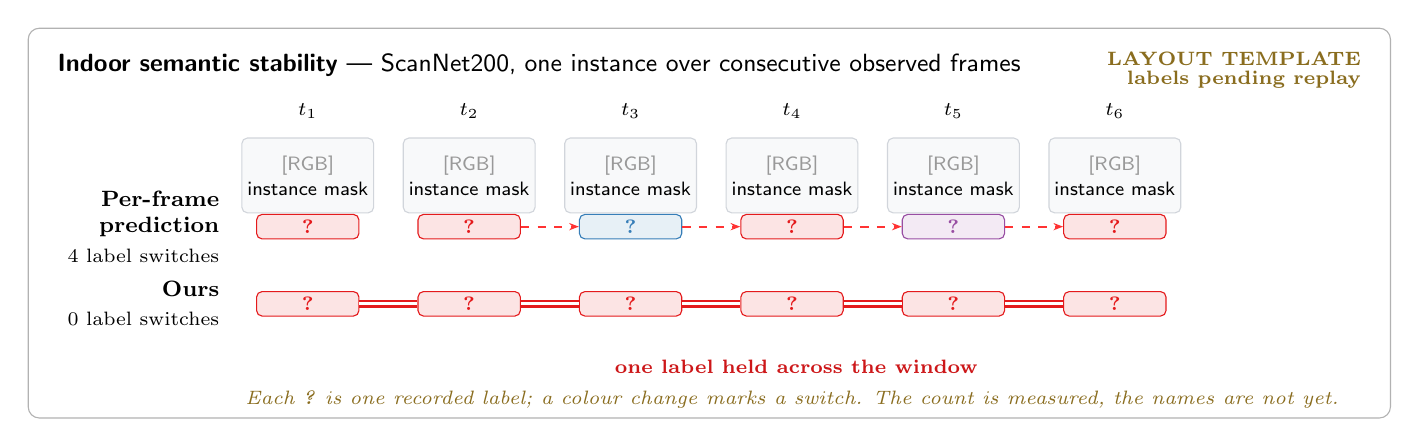
\begin{tikzpicture}[
    font=\small\sffamily,
    framebox/.style={draw=bordergray, fill=boxbg, rounded corners=2pt, minimum width=1.55cm, minimum height=0.95cm, align=center, inner sep=2pt},
    lab/.style={rounded corners=2pt, font=\scriptsize\bfseries, inner sep=2pt, minimum width=1.30cm, align=center},
    labA/.style={lab, fill=idred!12,    text=idred,    draw=idred},
    labB/.style={lab, fill=idblue!12,   text=idblue,   draw=idblue},
    labC/.style={lab, fill=idpurple!12, text=idpurple, draw=idpurple},
    labD/.style={lab, fill=idorange!14, text=idorange!75!black, draw=idorange},
    subpanel/.style={draw=black!30, fill=white, rounded corners=4pt}
]
% ---------------- header ----------------
\node[anchor=north west, font=\small\sffamily] (title) at (0.25, -0.2)
  {\textbf{Indoor semantic stability} --- ScanNet200, one instance over consecutive observed frames};
\node[anchor=north east, font=\scriptsize\bfseries, text=pend, align=right] at (17.05, -0.18)
  {LAYOUT TEMPLATE\\[-1pt]labels pending replay};
% ---------------- frame strip ----------------
\foreach \i/\t in {0/{$t_1$}, 1/{$t_2$}, 2/{$t_3$}, 3/{$t_4$}, 4/{$t_5$}, 5/{$t_6$}} {
    \node[anchor=center, font=\scriptsize\bfseries] (time\i) at (3.55 + \i*2.05, -1.05) {\t};
    \node[framebox, below=0.12cm of time\i] (frame\i) {
        \textcolor{gray!80}{\scriptsize [RGB]}\\[-2pt]
        \scriptsize instance mask
    };
}
% ---------------- rows ----------------
\node[anchor=east, align=right, font=\footnotesize] (lblBase) at (2.55, -2.52)
  {\textbf{Per-frame}\\\textbf{prediction}\\[1pt]{\scriptsize 4 label switches}};
\node[anchor=east, align=right, font=\footnotesize] (lblOurs) at (2.55, -3.50)
  {\textbf{Ours}\\[1pt]{\scriptsize 0 label switches}};
% baseline row: 5 label runs == the measured 4 switches. Identity of each run unknown.
% 6 cells, 4 switches (the measured count): A A | B | A | C | A
\node[labA] (b0) at (frame0 |- lblBase) {?};
\node[labA] (b1) at (frame1 |- lblBase) {?};
\node[labB] (b2) at (frame2 |- lblBase) {?};
\node[labA] (b3) at (frame3 |- lblBase) {?};
\node[labC] (b4) at (frame4 |- lblBase) {?};
\node[labA] (b5) at (frame5 |- lblBase) {?};
\foreach \a/\b in {b1/b2, b2/b3, b3/b4, b4/b5}
  \draw[-{Stealth[length=3.5pt]}, dashed, red!80, line width=0.8pt] (\a) -- (\b);
% ours row: one label, held
\foreach \i in {0,...,5} \node[labA] (o\i) at (frame\i |- lblOurs) {?};
\draw[double, double distance=1.2pt, idred, line width=0.9pt] (o0) -- (o1) -- (o2) -- (o3) -- (o4) -- (o5);
\node[anchor=center, font=\scriptsize\bfseries\color{idred!90!black}] at (9.7, -4.30)
  {$\checkmark$ one label held across the window};
\node[anchor=center, font=\scriptsize\itshape\color{pend}] at (9.7, -4.72)
  {Each \textbf{?} is one recorded label; a colour change marks a switch. The count is measured, the names are not yet.};
\begin{scope}[on background layer]
    \draw[subpanel] (0, 0) rectangle (17.3, -4.95);
\end{scope}
\end{tikzpicture}
\caption{\textbf{LAYOUT TEMPLATE --- not yet a result.}
Intended structure of the indoor figure: one instance, consecutive observed frames, the per-frame open-vocabulary prediction above and our emitted label below.
The number of label runs shown matches the measured switch count for the candidate instance; the class names are deliberately left as \textbf{?} because no stored run persists the per-frame label sequence, and recovering it requires a replay that has not been run.
Candidate instances, with measured switch count, track length and mask IoU, are listed in the accompanying shortlist; the chosen one fills this layout unchanged.}
\label{fig:semantic_stability}
\end{figure*}

% Drawn at 17.3cm == \textwidth (6.875in = 17.46cm) -- do NOT wrap in \resizebox.
\usetikzlibrary{positioning, arrows.meta, backgrounds, fit}

\definecolor{idred}{HTML}{E41A1C}
\definecolor{idblue}{HTML}{377EB8}
\definecolor{idpurple}{HTML}{984EA3}
\definecolor{idorange}{HTML}{FF7F00}
\definecolor{boxbg}{HTML}{F8F9FA}
\definecolor{bordergray}{HTML}{D1D5DB}
\definecolor{pend}{HTML}{8A6D1F}

\begin{figure*}[t]
\centering
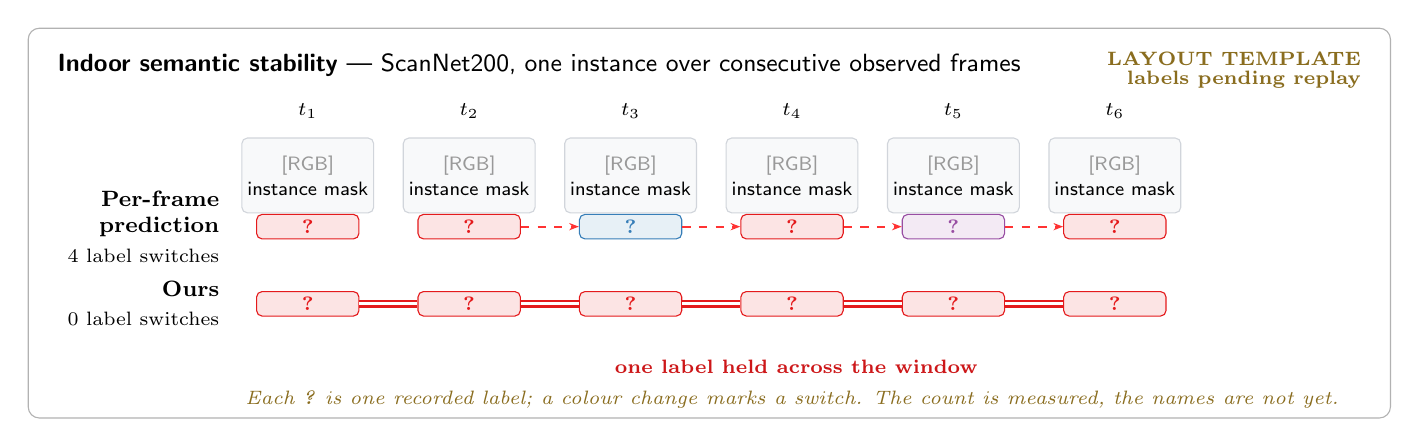
\begin{tikzpicture}[
    font=\small\sffamily,
    framebox/.style={draw=bordergray, fill=boxbg, rounded corners=2pt, minimum width=1.55cm, minimum height=0.95cm, align=center, inner sep=2pt},
    lab/.style={rounded corners=2pt, font=\scriptsize\bfseries, inner sep=2pt, minimum width=1.30cm, align=center},
    labA/.style={lab, fill=idred!12,    text=idred,    draw=idred},
    labB/.style={lab, fill=idblue!12,   text=idblue,   draw=idblue},
    labC/.style={lab, fill=idpurple!12, text=idpurple, draw=idpurple},
    labD/.style={lab, fill=idorange!14, text=idorange!75!black, draw=idorange},
    subpanel/.style={draw=black!30, fill=white, rounded corners=4pt}
]
% ---------------- header ----------------
\node[anchor=north west, font=\small\sffamily] (title) at (0.25, -0.2)
  {\textbf{Indoor semantic stability} --- ScanNet200, one instance over consecutive observed frames};
\node[anchor=north east, font=\scriptsize\bfseries, text=pend, align=right] at (17.05, -0.18)
  {LAYOUT TEMPLATE\\[-1pt]labels pending replay};
% ---------------- frame strip ----------------
\foreach \i/\t in {0/{$t_1$}, 1/{$t_2$}, 2/{$t_3$}, 3/{$t_4$}, 4/{$t_5$}, 5/{$t_6$}} {
    \node[anchor=center, font=\scriptsize\bfseries] (time\i) at (3.55 + \i*2.05, -1.05) {\t};
    \node[framebox, below=0.12cm of time\i] (frame\i) {
        \textcolor{gray!80}{\scriptsize [RGB]}\\[-2pt]
        \scriptsize instance mask
    };
}
% ---------------- rows ----------------
\node[anchor=east, align=right, font=\footnotesize] (lblBase) at (2.55, -2.52)
  {\textbf{Per-frame}\\\textbf{prediction}\\[1pt]{\scriptsize 4 label switches}};
\node[anchor=east, align=right, font=\footnotesize] (lblOurs) at (2.55, -3.50)
  {\textbf{Ours}\\[1pt]{\scriptsize 0 label switches}};
% baseline row: 5 label runs == the measured 4 switches. Identity of each run unknown.
% 6 cells, 4 switches (the measured count): A A | B | A | C | A
\node[labA] (b0) at (frame0 |- lblBase) {?};
\node[labA] (b1) at (frame1 |- lblBase) {?};
\node[labB] (b2) at (frame2 |- lblBase) {?};
\node[labA] (b3) at (frame3 |- lblBase) {?};
\node[labC] (b4) at (frame4 |- lblBase) {?};
\node[labA] (b5) at (frame5 |- lblBase) {?};
\foreach \a/\b in {b1/b2, b2/b3, b3/b4, b4/b5}
  \draw[-{Stealth[length=3.5pt]}, dashed, red!80, line width=0.8pt] (\a) -- (\b);
% ours row: one label, held
\foreach \i in {0,...,5} \node[labA] (o\i) at (frame\i |- lblOurs) {?};
\draw[double, double distance=1.2pt, idred, line width=0.9pt] (o0) -- (o1) -- (o2) -- (o3) -- (o4) -- (o5);
\node[anchor=center, font=\scriptsize\bfseries\color{idred!90!black}] at (9.7, -4.30)
  {$\checkmark$ one label held across the window};
\node[anchor=center, font=\scriptsize\itshape\color{pend}] at (9.7, -4.72)
  {Each \textbf{?} is one recorded label; a colour change marks a switch. The count is measured, the names are not yet.};
\begin{scope}[on background layer]
    \draw[subpanel] (0, 0) rectangle (17.3, -4.95);
\end{scope}
\end{tikzpicture}
\caption{\textbf{LAYOUT TEMPLATE --- not yet a result.}
Intended structure of the indoor figure: one instance, consecutive observed frames, the per-frame open-vocabulary prediction above and our emitted label below.
The number of label runs shown matches the measured switch count for the candidate instance; the class names are deliberately left as \textbf{?} because no stored run persists the per-frame label sequence, and recovering it requires a replay that has not been run.
Candidate instances, with measured switch count, track length and mask IoU, are listed in the accompanying shortlist; the chosen one fills this layout unchanged.}
\label{fig:semantic_stability}
\end{figure*}

% Drawn at 17.3cm == \textwidth (6.875in = 17.46cm) -- do NOT wrap in \resizebox.
\usetikzlibrary{positioning, arrows.meta, backgrounds, fit}

\definecolor{idred}{HTML}{E41A1C}
\definecolor{idblue}{HTML}{377EB8}
\definecolor{idpurple}{HTML}{984EA3}
\definecolor{idorange}{HTML}{FF7F00}
\definecolor{boxbg}{HTML}{F8F9FA}
\definecolor{bordergray}{HTML}{D1D5DB}
\definecolor{pend}{HTML}{8A6D1F}

\begin{figure*}[t]
\centering
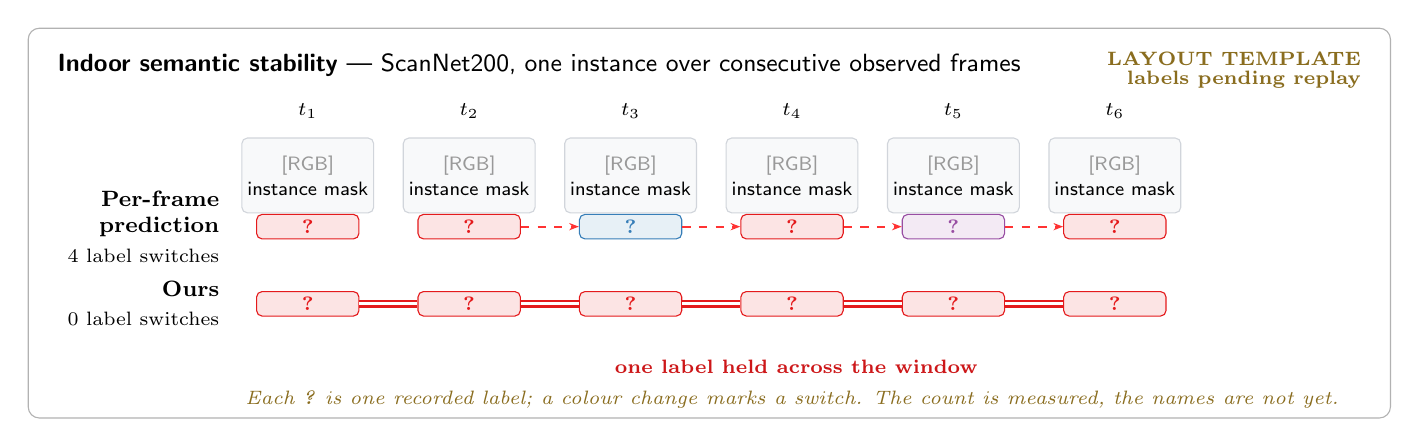
\begin{tikzpicture}[
    font=\small\sffamily,
    framebox/.style={draw=bordergray, fill=boxbg, rounded corners=2pt, minimum width=1.55cm, minimum height=0.95cm, align=center, inner sep=2pt},
    lab/.style={rounded corners=2pt, font=\scriptsize\bfseries, inner sep=2pt, minimum width=1.30cm, align=center},
    labA/.style={lab, fill=idred!12,    text=idred,    draw=idred},
    labB/.style={lab, fill=idblue!12,   text=idblue,   draw=idblue},
    labC/.style={lab, fill=idpurple!12, text=idpurple, draw=idpurple},
    labD/.style={lab, fill=idorange!14, text=idorange!75!black, draw=idorange},
    subpanel/.style={draw=black!30, fill=white, rounded corners=4pt}
]
% ---------------- header ----------------
\node[anchor=north west, font=\small\sffamily] (title) at (0.25, -0.2)
  {\textbf{Indoor semantic stability} --- ScanNet200, one instance over consecutive observed frames};
\node[anchor=north east, font=\scriptsize\bfseries, text=pend, align=right] at (17.05, -0.18)
  {LAYOUT TEMPLATE\\[-1pt]labels pending replay};
% ---------------- frame strip ----------------
\foreach \i/\t in {0/{$t_1$}, 1/{$t_2$}, 2/{$t_3$}, 3/{$t_4$}, 4/{$t_5$}, 5/{$t_6$}} {
    \node[anchor=center, font=\scriptsize\bfseries] (time\i) at (3.55 + \i*2.05, -1.05) {\t};
    \node[framebox, below=0.12cm of time\i] (frame\i) {
        \textcolor{gray!80}{\scriptsize [RGB]}\\[-2pt]
        \scriptsize instance mask
    };
}
% ---------------- rows ----------------
\node[anchor=east, align=right, font=\footnotesize] (lblBase) at (2.55, -2.52)
  {\textbf{Per-frame}\\\textbf{prediction}\\[1pt]{\scriptsize 4 label switches}};
\node[anchor=east, align=right, font=\footnotesize] (lblOurs) at (2.55, -3.50)
  {\textbf{Ours}\\[1pt]{\scriptsize 0 label switches}};
% baseline row: 5 label runs == the measured 4 switches. Identity of each run unknown.
% 6 cells, 4 switches (the measured count): A A | B | A | C | A
\node[labA] (b0) at (frame0 |- lblBase) {?};
\node[labA] (b1) at (frame1 |- lblBase) {?};
\node[labB] (b2) at (frame2 |- lblBase) {?};
\node[labA] (b3) at (frame3 |- lblBase) {?};
\node[labC] (b4) at (frame4 |- lblBase) {?};
\node[labA] (b5) at (frame5 |- lblBase) {?};
\foreach \a/\b in {b1/b2, b2/b3, b3/b4, b4/b5}
  \draw[-{Stealth[length=3.5pt]}, dashed, red!80, line width=0.8pt] (\a) -- (\b);
% ours row: one label, held
\foreach \i in {0,...,5} \node[labA] (o\i) at (frame\i |- lblOurs) {?};
\draw[double, double distance=1.2pt, idred, line width=0.9pt] (o0) -- (o1) -- (o2) -- (o3) -- (o4) -- (o5);
\node[anchor=center, font=\scriptsize\bfseries\color{idred!90!black}] at (9.7, -4.30)
  {$\checkmark$ one label held across the window};
\node[anchor=center, font=\scriptsize\itshape\color{pend}] at (9.7, -4.72)
  {Each \textbf{?} is one recorded label; a colour change marks a switch. The count is measured, the names are not yet.};
\begin{scope}[on background layer]
    \draw[subpanel] (0, 0) rectangle (17.3, -4.95);
\end{scope}
\end{tikzpicture}
\caption{\textbf{LAYOUT TEMPLATE --- not yet a result.}
Intended structure of the indoor figure: one instance, consecutive observed frames, the per-frame open-vocabulary prediction above and our emitted label below.
The number of label runs shown matches the measured switch count for the candidate instance; the class names are deliberately left as \textbf{?} because no stored run persists the per-frame label sequence, and recovering it requires a replay that has not been run.
Candidate instances, with measured switch count, track length and mask IoU, are listed in the accompanying shortlist; the chosen one fills this layout unchanged.}
\label{fig:semantic_stability}
\end{figure*}

% Drawn at 17.3cm == \textwidth (6.875in = 17.46cm) -- do NOT wrap in \resizebox.
\usetikzlibrary{positioning, arrows.meta, backgrounds, fit}

\definecolor{idred}{HTML}{E41A1C}
\definecolor{idblue}{HTML}{377EB8}
\definecolor{idpurple}{HTML}{984EA3}
\definecolor{idorange}{HTML}{FF7F00}
\definecolor{boxbg}{HTML}{F8F9FA}
\definecolor{bordergray}{HTML}{D1D5DB}
\definecolor{pend}{HTML}{8A6D1F}

\begin{figure*}[t]
\centering
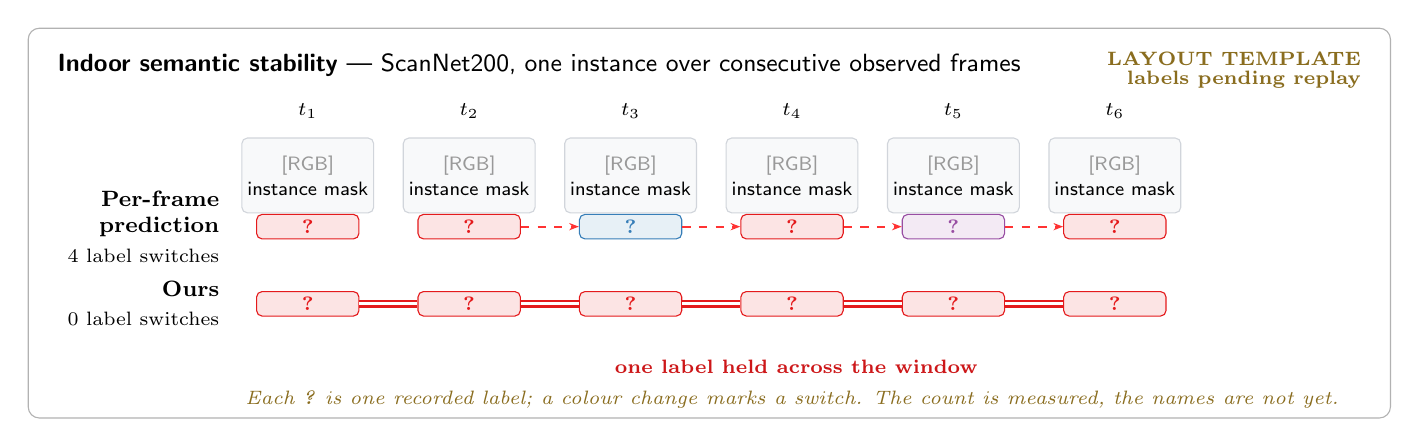
\begin{tikzpicture}[
    font=\small\sffamily,
    framebox/.style={draw=bordergray, fill=boxbg, rounded corners=2pt, minimum width=1.55cm, minimum height=0.95cm, align=center, inner sep=2pt},
    lab/.style={rounded corners=2pt, font=\scriptsize\bfseries, inner sep=2pt, minimum width=1.30cm, align=center},
    labA/.style={lab, fill=idred!12,    text=idred,    draw=idred},
    labB/.style={lab, fill=idblue!12,   text=idblue,   draw=idblue},
    labC/.style={lab, fill=idpurple!12, text=idpurple, draw=idpurple},
    labD/.style={lab, fill=idorange!14, text=idorange!75!black, draw=idorange},
    subpanel/.style={draw=black!30, fill=white, rounded corners=4pt}
]
% ---------------- header ----------------
\node[anchor=north west, font=\small\sffamily] (title) at (0.25, -0.2)
  {\textbf{Indoor semantic stability} --- ScanNet200, one instance over consecutive observed frames};
\node[anchor=north east, font=\scriptsize\bfseries, text=pend, align=right] at (17.05, -0.18)
  {LAYOUT TEMPLATE\\[-1pt]labels pending replay};
% ---------------- frame strip ----------------
\foreach \i/\t in {0/{$t_1$}, 1/{$t_2$}, 2/{$t_3$}, 3/{$t_4$}, 4/{$t_5$}, 5/{$t_6$}} {
    \node[anchor=center, font=\scriptsize\bfseries] (time\i) at (3.55 + \i*2.05, -1.05) {\t};
    \node[framebox, below=0.12cm of time\i] (frame\i) {
        \textcolor{gray!80}{\scriptsize [RGB]}\\[-2pt]
        \scriptsize instance mask
    };
}
% ---------------- rows ----------------
\node[anchor=east, align=right, font=\footnotesize] (lblBase) at (2.55, -2.52)
  {\textbf{Per-frame}\\\textbf{prediction}\\[1pt]{\scriptsize 4 label switches}};
\node[anchor=east, align=right, font=\footnotesize] (lblOurs) at (2.55, -3.50)
  {\textbf{Ours}\\[1pt]{\scriptsize 0 label switches}};
% baseline row: 5 label runs == the measured 4 switches. Identity of each run unknown.
% 6 cells, 4 switches (the measured count): A A | B | A | C | A
\node[labA] (b0) at (frame0 |- lblBase) {?};
\node[labA] (b1) at (frame1 |- lblBase) {?};
\node[labB] (b2) at (frame2 |- lblBase) {?};
\node[labA] (b3) at (frame3 |- lblBase) {?};
\node[labC] (b4) at (frame4 |- lblBase) {?};
\node[labA] (b5) at (frame5 |- lblBase) {?};
\foreach \a/\b in {b1/b2, b2/b3, b3/b4, b4/b5}
  \draw[-{Stealth[length=3.5pt]}, dashed, red!80, line width=0.8pt] (\a) -- (\b);
% ours row: one label, held
\foreach \i in {0,...,5} \node[labA] (o\i) at (frame\i |- lblOurs) {?};
\draw[double, double distance=1.2pt, idred, line width=0.9pt] (o0) -- (o1) -- (o2) -- (o3) -- (o4) -- (o5);
\node[anchor=center, font=\scriptsize\bfseries\color{idred!90!black}] at (9.7, -4.30)
  {$\checkmark$ one label held across the window};
\node[anchor=center, font=\scriptsize\itshape\color{pend}] at (9.7, -4.72)
  {Each \textbf{?} is one recorded label; a colour change marks a switch. The count is measured, the names are not yet.};
\begin{scope}[on background layer]
    \draw[subpanel] (0, 0) rectangle (17.3, -4.95);
\end{scope}
\end{tikzpicture}
\caption{\textbf{LAYOUT TEMPLATE --- not yet a result.}
Intended structure of the indoor figure: one instance, consecutive observed frames, the per-frame open-vocabulary prediction above and our emitted label below.
The number of label runs shown matches the measured switch count for the candidate instance; the class names are deliberately left as \textbf{?} because no stored run persists the per-frame label sequence, and recovering it requires a replay that has not been run.
Candidate instances, with measured switch count, track length and mask IoU, are listed in the accompanying shortlist; the chosen one fills this layout unchanged.}
\label{fig:semantic_stability}
\end{figure*}
